%=================================================================
\section{Introduction}\label{sec-intro}


Emotion detection has attracted great interest 
in the natural language processing (NLP)
in the last few years.
In sentiment analysis, 
affective states are generally represented 
using either categorical or dimensional approaches.
The most popular categorical approach represents is 
Ekman’s six basic emotions 
(e.g., anger, happiness, fear, sadness, disgust and surprise)
The dimensional approach represents affective states by using
continuous numerical values in two/three dimensions,.
The valence-arousal (VA) dimensions model , 
as shown in ~\Cref{fig:va}. 
The valence represents the degree of 
positive and negative, 
while the arousal represents the degree of 
excitement and calm. 
In 1994,
Bradley and Lang proposed 
Valence- Arousal-Dominance model,
as shown in ~\Cref{fig:vad}.
And Dominance perceived degree of control in a (social) situation.
Based on this representation, 
any affective state can be represented as a point 
in the VA/VAD coordinate plane. 
Based on this representation, 
any affective state can be represented as 
a point in the VA/VAD coordinate plane.

In this paper, 
we want to predict  
multiple emotion dimension scores for an input text.
A new machine learning paradigm called 
Label Distribution Learning (LDL) 
was proposed in recently years.
Similarly,
we propose an dimensional emotion distribution learning (DEDL) algorithm
Different from the previous approaches, 
DEDL assumes that
each sentence contains a mixture of 
dimensional emotions with different intensities. 
We can label each sentence with 
an label distribution vector 
where elements corresponds to 
dimensional emotions and 
the value of each element indicates the intensity of the dimensional emotions. 
We require that each vector element has a value 
between 0 and 1 and they sum up to 1.

Use Dimensional EmotionS Distribution Learning
to predict multiple emotion dimension scores for an input text.
Then use the predicted VAD and notational VAD to 
do emotion classification.
Also, 
we will use the Deep Learning to do emotion classifiction.

\begin{figure}[htbp]
	\begin{minipage}[t]{0.5\linewidth}
		\centering
		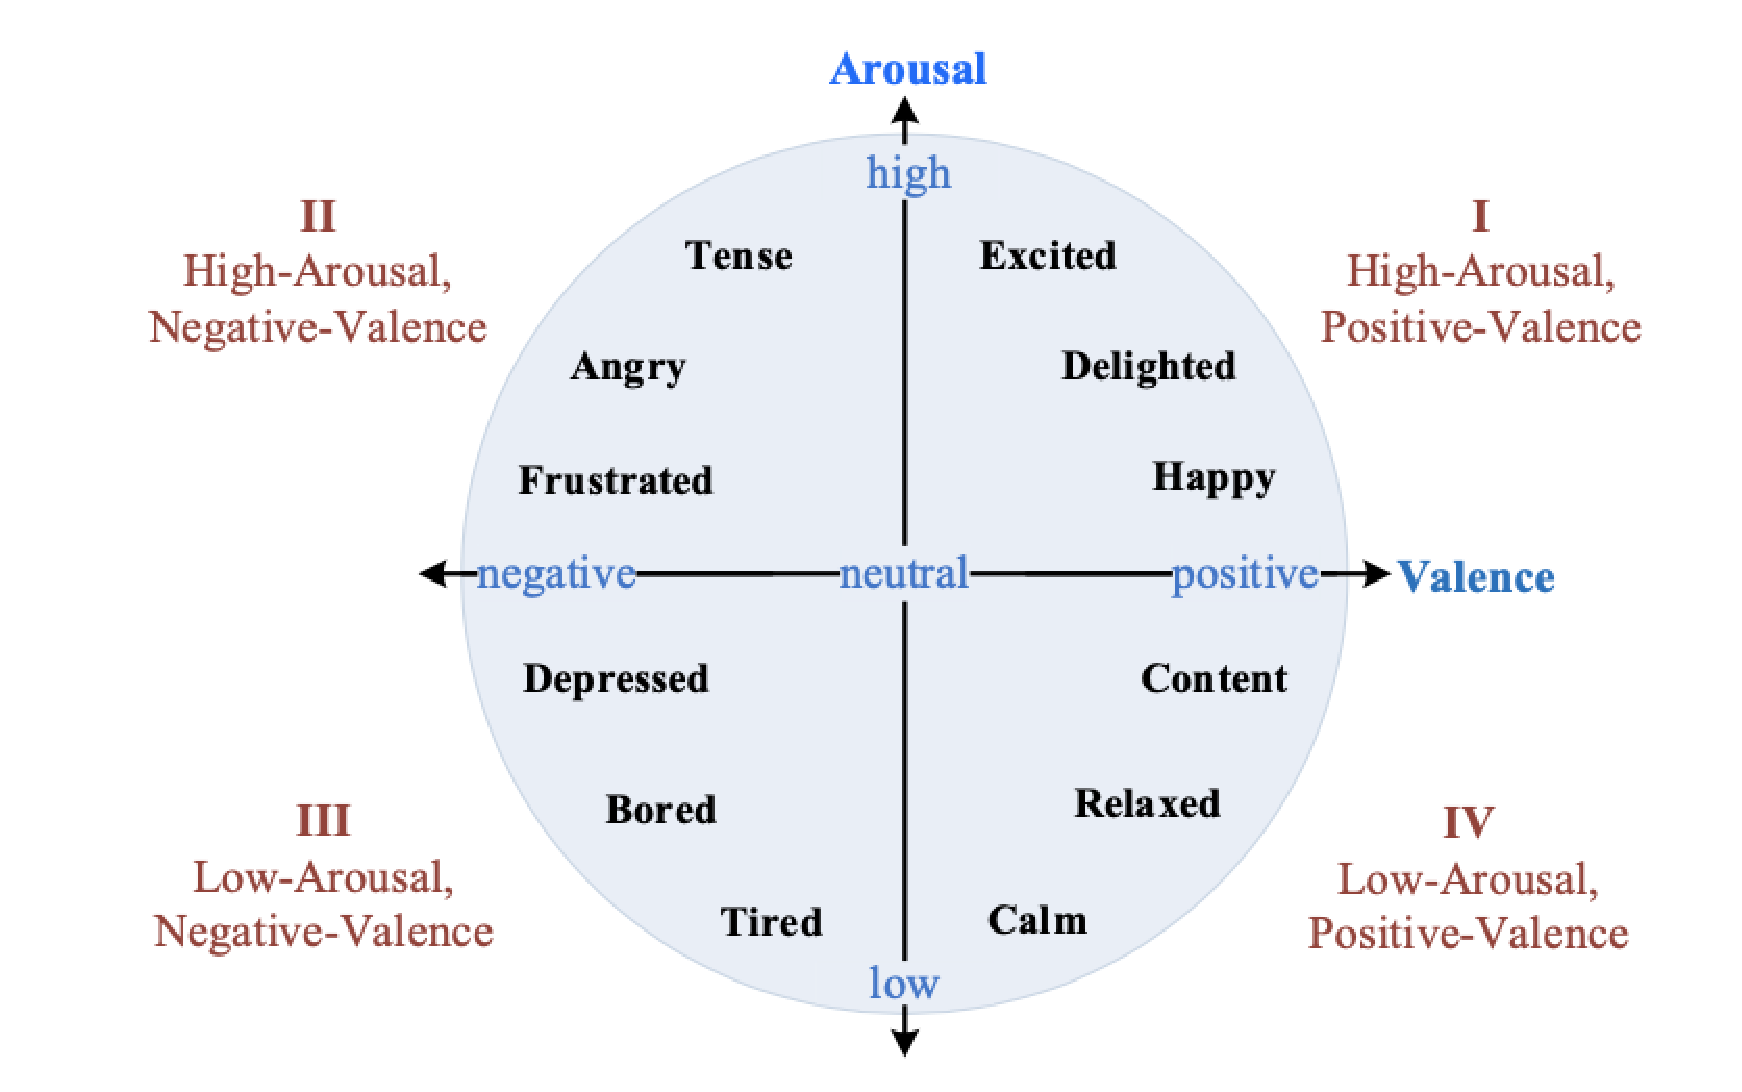
\includegraphics[height=4cm,width=6cm]{figures/va_emotion.eps}
		\caption{The emotional space spanned by the Valence-Arousal model}\label{fig:va}
	\end{minipage}%
	\hfill
	\begin{minipage}[t]{0.5\linewidth}
		\centering
		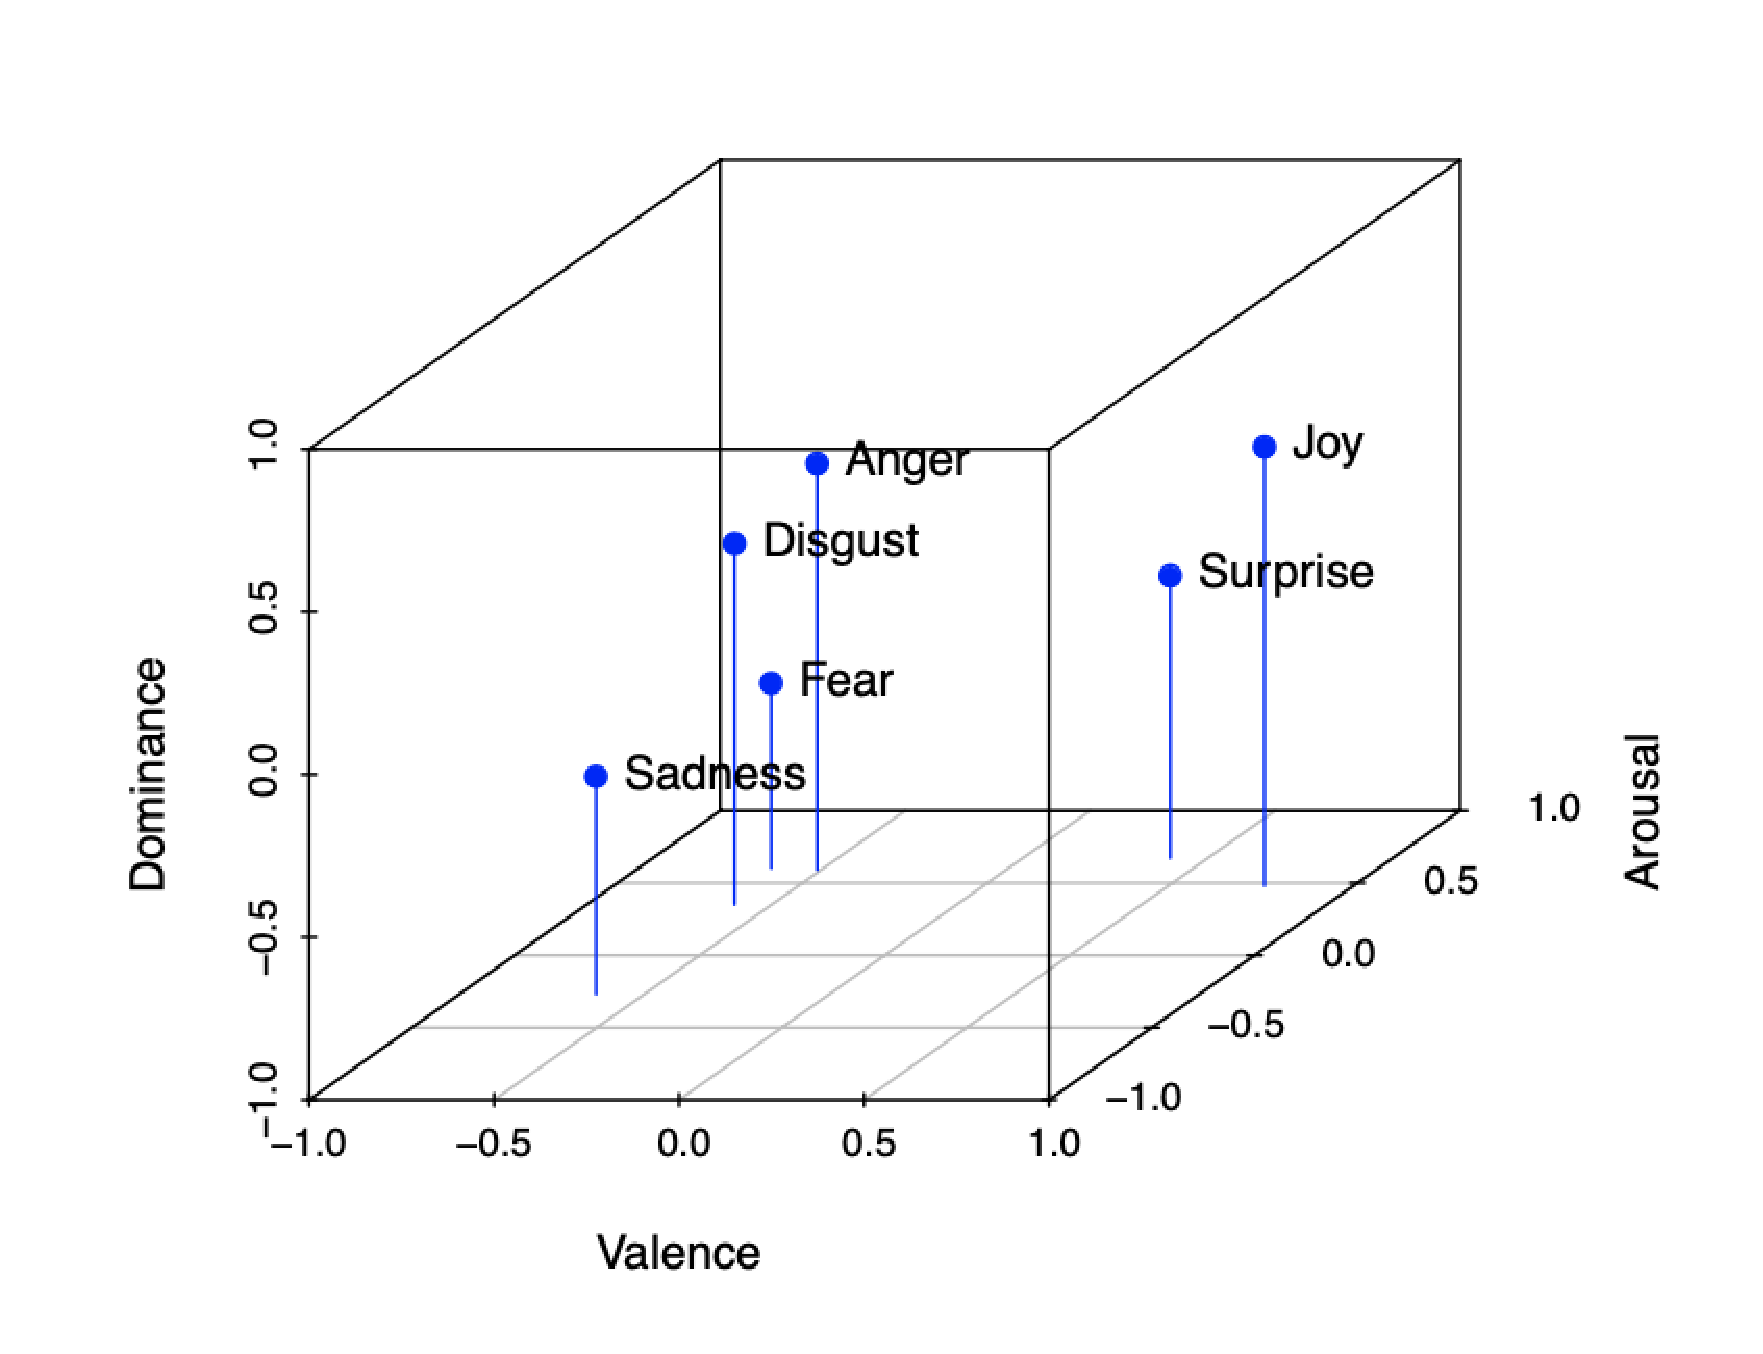
\includegraphics[height=4cm,width=6cm]{figures/six_emotions_vad.eps}
		\caption{The emotional space spanned by the Valence-Arousal-Dominance model. }\label{fig:vad}
	\end{minipage}
\end{figure}

%%==========================================================================================
%%

\section{Related Work}

\subsection{Emotion Frameworks}
\

Two main approaches of emotion representation exist, 
namely categorical approaches and dimensional approaches.
In the categorical approach, 
emotions are represented as specific discrete categories.
 Ekman’s (1992) theory of six basic emotions 
 (joy, sadness, anger, fear, disgust, and surprise) 
 is the most well-known, 
 but also Plutchik’s (1980) wheel of emotions, 
 in which joy, sadness, anger, fear, disgust, surprise, trust, 
 and anticipation are considered most basic,
is a common framework in emotion studies. 
However, 
many other theorists provide basic emotion frameworks, 
which can count up to fourteen emotion categories 
(Izard 1971; Roseman 1984).

In dimensional models, 
emotions are represented as a point in a multidimensional space. 
According to Mehrabian and Russell (1974), 
every emotional state can be described by 
scores on the dimensions valence (unhappiness-happiness), 
arousal (calmness-excitement) and dominance (submission-dominance),
known as the VAD-model. 
However, 
in later work Russell (1980) argued that 
the two dimensions valence and arousal suffice 
for describing emotional states, 
whereas Fontaine et al. (2007) suggest adding a fourth dimension: 
unpredictability.


%%==========================================================================================
%%

\subsection{Label Distribution Learning}
\

In the LDL framework, 
each instance is labeled by a real-valued vector
The goal of LDL is to 
predict multiple real-valued description degrees of the labels.
The instance variable is denoted by $ x $ , 
the particular \textit{i}-th instant is denoted by $ x_{i} $, 
the label variable is denoted by $ y $,
the particular \textit{j}-th label value is denoted by $ y_{j} $, 
the description degree of $ y $ to $ x $ is denoted by $ d ^ y_{x} $, 
and the label distribution of $ x $ is denoted by 
$  D_{i}  = \{ d^{{y_{1}} }_{ x_{i} }, d^{{y_{2}} }_{ x_{i} },...,d^{{y_{c}} }_{ x_{i} } \} $,
where $ c $ is the number of possible label values
and $ \sum_{y}  d^y_{x} = 1 $.
$ d^y_{x}  $ can be represented by 
the form of conditional probability, i.e., 
$ d^y_{x} =  P (y|x)$. 

Suppose $ p(y|x) $  is a parametric model
$ p(y|x;{\theta}) $, 
where $ \theta $ is the parameter vector. 
Given the training set $ S $, 
the goal of LDL is to find the $ /theta $ that 
can generate a distribution similar to $ D_{i} $
given the instance $ x_{i} $.
As for the Kullback-Leibler divergence,

\begin{equation}\label{eq:kl_divergence}
\theta^{\ast} =
\mathop{\arg\min}\limits_{\theta}
\sum\limits_{i}
\sum\limits_{j}
(d^{y_{j}}_{ x_{ i } }
\ln \dfrac{ d^{y_{j}}_{ x_{ i } } }{ p( y_{ j } | x_{ i } ;{\theta}) })
\end{equation}

Assumes the parametric model 
$ p(y|x;{\theta}) $ 
to be the maximum entropy model,	

\begin{equation}\label{eq:max_entropy}
	p(y|x;{\theta}) = \dfrac{1}{Z}
	\exp ( \sum\limits_{k}
	{\theta}_{y,k} 
	g_{k}( \textbf{x})  )
\end{equation}

where $ Z = \sum _{y}
\sum_{k}  {\theta}_{y,k}  g_{k}( \textbf{x}) $
is a normalization factor,
$ {\theta}_{y,k} $ is an element in \textbf {$\theta$} ,
and $ g_{k}( \textbf{x}) $ is the \textit{k}-th feature of\textbf{ x}.
Use a strategy similar to Improved Iterative Scaling (IIS) 
to find the best answer.

%%==========================================================================================
%%
\section{Data Set}


%\section{Preliminaries} \label{sec-preliminaries}

\blindtext

\gliMarker  %TODO: GLi Here


\section{Method} \label{sec-method}

\blindtext
\blindlist{itemize}[3]
\blinditemize
\blindenumerate

\blindmathtrue
\blindmathfalse
\blinddescription

\sxlinMarker %TODO: QWu Here

\section{Experiment and Analysis} \label{sec-experiment}


\begin{table}  \centering
  \caption{Precision Comparison on Event Detection Methods}
  \label{tbl:overall-experiments}
  \begin{tabular}{cccc}
\toprule
    % after \\: \hline or \cline{col1-col2} \cline{col3-col4} ...
    & OR Event Detection & AC Event Detection & TC Event Detection \\
\midrule
    precision & 0.83 & 0.69 & 0.46 \\
    recall & 0.68 & 0.48 & 0.36 \\
    F-score & 0.747 & 0.57 & 0.4 \\
\bottomrule
\end{tabular}
\end{table}


\section{Conclusions} \label{sec-conclusions}

\blindtext

\section*{Acknowledgment}

\lipsum[1]


The authors would like to thank \ldots

